\documentclass[b5paper, 12pt]{article}
\usepackage[inner=0.9in, outer=0.9in, top=80pt, bottom=0.76in]{geometry}
\usepackage{adjustbox}
\usepackage{tcolorbox} % ボックス作成
\usepackage{ulem}
\usepackage{soul}
\usepackage{lipsum} 
\usepackage{setspace} 
\usepackage{comment}
\usepackage{letterspace}
\usepackage{tikz} % 図形描画用
\usepackage{subfig} % 画像を並べるのに便利なパッケージ
\usetikzlibrary{math}
\usepackage{ifthen}
\usepackage{multicol}
\usepackage{tabularx}
\usepackage{booktabs}
\usepackage{enumitem}
\usepackage{amsmath, amssymb} % 数式関連
\usepackage{relsize} % プリアンブルに追加
\usepackage{mathabx}
\usepackage{mathtools}
\usepackage{mathcomp}
\usepackage{siunitx}
\usetikzlibrary{calc}
\usepackage{pgffor}
\usepackage{pifont}
\usepackage{graphicx} % 画像関連
\graphicspath{{Images/}}
\usepackage{caption}
\captionsetup{justification=raggedright, singlelinecheck=false, font=scriptsize}
\usepackage{fancyhdr} % ヘッダー・フッター
\usepackage{titlesec} % セクションのスタイル調整
\usepackage{parskip} % 段落間のスペース調整
\usepackage{luatexja} % LuaLaTeX での日本語処理
\usepackage{luatexja-preset}
\usepackage{luatexja-fontspec} 
\usepackage{xcolor}  
\usepackage{fontspec} % フォント指定
\usepackage{url} % URL を扱うためのパッケージ
\usepackage[colorlinks=true, linkcolor=blue, urlcolor=blue]{hyperref}
\usepackage{array}
\usepackage{transparent}
\usepackage{changepage}
\usepackage{lipsum}   % ダミーテキスト（テスト用）

\definecolor{beige}{RGB}{252, 252, 252} % 肌色っぽいベージュ
\pagecolor{beige}
\linespread{1.5}
\setmainfont[
    Scale=1.1,
]{Times New Roman}
\setmainjfont[
    Scale=1.0,
    Weight=2,
    Renderer=Harfbuzz, % Harfbuzzレンダラーを使用
    LetterSpace=11
]{Hiragino Mincho ProN}
\setsansjfont{Hiragino Kaku Gothic ProN W3}


\pagestyle{fancy}  % ヘッダー・フッターをカスタマイズ
\fancyhf{}
\renewcommand{\headrulewidth}{0pt} % ヘッダーの横線を非表示
\renewcommand{\footrulewidth}{0pt} % フッターの横線を非表示
% 表紙（plain スタイル）のとき、フッターを空にする
\fancypagestyle{plain}{%
    \fancyhf{}
}
% ページ番号のフォーマット
\fancyfoot[C]{\raisebox{40mm}{\fontsize{10pt}{11pt}\selectfont\textemdash\hspace{0.55em}\thepage\hspace{0.55em}\textemdash}}
\def\toFullWidth#1{\char\numexpr "FF10 + #1\relax}

\tikzmath{
  function calc_index(\h, \w, \count) {
    return int((\count div \h) + \w * (\count mod \h) + 1);
  };
}

\setul{1pt}{0.4em} % 1pt が線の太さ, 0.4em が線と文字の間隔

\newcounter{mondai} % 問題番号のカウンターを作成
\setcounter{mondai}{0} % カウンターの初期化
\newcommand{\nextmondai}{
    \stepcounter{mondai} % カウンターを1つ増やす
    \noindent\textsf{\textbf{\Large 第\toFullWidth{\arabic{mondai}}問}} \hspace{0.5em}
}
\newcommand{\egg}[1]{\,\raisebox{-3 pt}{
  \begin{tikzpicture}[x = 1 pt, y = 1 pt, line width = 1.1pt, scale = 1.0]
  \draw (0,0) ellipse (4.5 and 6);\draw (0.1,0.2) node{\small\usefont{T1}{qhv}{m}{n}{#1}};\end{tikzpicture}}\,}

\newcounter{boxcounter}
\setcounter{boxcounter}{0} % 初期値
\newcommand{\counterbox}[1][0em]{%
    \stepcounter{boxcounter}% カウンタをインクリメント
    \begin{tikzpicture}[scale=0.72]
        \begin{scope}[transform canvas={shift={(0em, \dimexpr -0.5em + #1\relax)}}] % 強制的に移動
            \draw[very thick] (0,0) rectangle (2.3,1.1); % 長方形の枠
            \node[fill=beige] at (1.15,0.55) {\theboxcounter}; % 数字を中央に配置
        \end{scope}
    \end{tikzpicture}%
}

\newcommand{\haiten}[1]{
    \textcolor{black!70}{\;（配点\quad\!\!#1）}
}

\begin{comment}
    1. 方程式クイズ
    2. 暗殺教室
    3. シュタゲ
    4. ベン図クイズ。
    5. 漢字クイズ
    6. 不等式
    7, 口コミクイズ
    8. 英英辞典。
    9. 英文クイズ
\end{comment}

%-----------------------------------------表紙-------------------------------------------------

\begin{document}
\pagenumbering{gobble} % 表紙はページ番号を表示しない
\begin{titlepage}
    \begin{tikzpicture}[remember picture, overlay]
        \node[anchor=north west, fill=black, minimum width=22pt, minimum height=10pt] 
            at ([yshift=-60pt]current page.north west) {};
    \end{tikzpicture}
\vspace{-3.5em}
\begin{center}
    \setlength{\fboxsep}{5pt}
    \fbox{\fontsize{11pt}{14pt}\selectfont\textbf{試験開始の指示があるまで， この問題冊子の中を見てはいけません。}}
\end{center}
\vspace{1.7em}
\hspace{1.0em}
\makebox[6.3cm][s]{\fontsize{27pt}{30pt}\textsf{漫画映画}}
\hfill
\makebox[0pt][r]{\raisebox{0.5em}{% ←ここで微調整
    \adjustbox{max width=50pt, max height=45pt}{$
        \left(\begin{array}{r}
            \text{\large 100点} \\[8pt]
            \text{\large 40分}
        \end{array}\right)
    $}
}}

\vspace{2.0em}
\makebox[7em][s]{\textbf{注意事項}}
% 注意事項のリスト
\begin{enumerate}[leftmargin=0em, label=\arabic*., itemsep=-5pt]
    \item 解答用紙に正しくマークされていない場合は, ~採点されないことがあります。
    \item この問題冊子は, ~全13ページで構成されています。問題は第1問から第9問まであり, ~
    一部の問題には小問が含まれます。配点は各問題ごとに明記されています。
    \item 試験中に問題冊子の印刷不鮮明，ページの落丁・乱丁及び問題の不備等に気付いた場合は教えてください。
    \item 解答は，各問題にある所定の記号をクリックまたはタップをしマークしなさい。
    以下の解答欄を用いて正常に動作することを確認しなさい。
\end{enumerate}
% 解答欄の例
\begin{table}[h]
    \centering
    \newcommand{\iibf}[1]{\!\egg{#1}\!}
    \newcommand{\eggfill}[1]{\,\raisebox{-3 pt}{ 
        \begin{tikzpicture}[x = 1 pt, y = 1 pt, line width = 1.1pt, scale = 1.0]
        \fill[gray, opacity=1.0] (0,0) ellipse (4.5 and 6);
        \draw (0,0) ellipse (4.5 and 6);\draw (0.1,0.2) node{\small\usefont{T1}{qhv}{m}{n}{#1}};\end{tikzpicture}}\,
    }
    \renewcommand{\arraystretch}{1.3}
    \begin{tabularx}{0.67\textwidth}{!{\vrule width 1.2pt} p{1.65cm}| X !{\vrule width 1.2pt}}
        \specialrule{1.2pt}{0pt}{0pt}
        \textsf{\textbf{\small 解答番号}} & \makebox[\hsize][s]{\textsf{\textbf{\small \hspace{2.5em}解答欄\hspace{2.5em}}}} \\  
        \hline
        \makebox[\hsize][c]{10} & \iibf{1}\iibf{2}\iibf{3}\iibf{4}\iibf{5}\iibf{6}\iibf{7}\iibf{8}\iibf{9} \\  
        \specialrule{1.2pt}{0pt}{0pt}
    \end{tabularx}
    \\
    % \eggfill{2} \quad
    % \eggfill{3} \quad
    % \eggfill{4} \quad
    % \eggfill{5} \quad 
    % \eggfill{6} \quad 
    % \eggfill{7} \quad 
    % \eggfill{8} \quad 
    % \eggfill{9} \quad 
\end{table}
% 注意事項続き
\begin{enumerate}[leftmargin=0em, label=\arabic*., resume, itemsep=-5pt]
    \item 試験中の他のウェブサイトおよび書籍等の閲覧は禁止します。
    \item 試験終了後, ~問題冊子は持ち帰りなさい。
    % \begin{enumerate}[label={}, leftmargin=0pt, itemsep=-5pt]
    %     \vspace*{-0.3em}
    %     \item ①\;不正行為に対しては厳正に対処します。
    %     \item ②\;不正行為に見えるような行為が見受けられた場合は，監督者がカードを用いて注意します。
    %     \item ③\;不正行為を行った場合は、その時点で受験を取りやめさせ退室させます。
    % \end{enumerate}
\end{enumerate}

\end{titlepage}
\clearpage 
% ---------------------------------------------------1---------------------------------------
\pagestyle{fancy}  % ここで適用し直す
\pagenumbering{arabic}
\newgeometry{inner=0.9in, outer=0.9in, top=50pt, bottom=0.76in}
\nextmondai
以下の連立方程式において, ~各式\;①\;\textasciitilde\;③\;が
それぞれ画像\;I\;\textasciitilde\;III\;に示されたアニメの名称の一部を表している。
このとき, ~式\;\:\scalebox{1.15}{\(n_d\:g'' atf\mathsmaller{-}\)}\;が表すアニメの名称として最も適当なものを, ~
次の\!\egg{1}\textasciitilde\!\egg{4}のうちから一つ選べ。
\hspace{0.6em}\counterbox[-0.15em]\hspace{4.0em}\haiten{10}\\
\vspace{-0.1em}
\begin{equation*}
    \Large
    \left\{\;\;
        \begin{aligned}
            y - x_n \;&=\; ci  \quad\quad &&\text{\small・・・\quad}\text{\large ①} \\
            fg'' \;&=\; c  \quad\quad &&\text{\small・・・\quad}\text{\large ②} \\
            pb \times abq\tcdegree \;&= _d \;t  \quad\quad &&\text{\small・・・\quad}\text{\large ③} \\
        \end{aligned}
    \right.
\end{equation*}
\par
\vspace{0.6em}
\begin{tikzpicture}[scale=0.45]
    % img1（左上の基準画像）
    \node[anchor=north west] (img1) at (-5,0) {\includegraphics[scale=0.25]{hibike.png}};
    % ラベル I
    \node[anchor=south west] at ([shift={(-0.2,0.12)}] img1.north west) {\textbf{\large I}};
    % \vspace*{1em}
    % img2（img1 の真下に配置）
    \node[anchor=north west] (img2) at ([xshift=-0.3em, yshift=-2.5cm] img1.south west) {\includegraphics[width=12.8em]{sidonia2.png}};
    % ラベル II
    \node[anchor=south west] at ([shift={(-0.2,0.12)}] img2.north west) {\textbf{\large II}};
    % img3（img1 の右に配置）
    \node[anchor=north west] (img3) at ([xshift=1.4cm] img1.north east) {\includegraphics[scale=0.55]{hurumetaru.png}};
    % ラベル III
    \node[anchor=south west] at ([shift={(-0.2,0.12)}] img3.north west) {\textbf{\large III}};
\end{tikzpicture}
\vspace{1.4em}
\begin{center}
    \hspace{-2.0em}
    \makebox[\textwidth]{
        \newcommand{\iibf}[1]{\!\egg{#1}\!}
        \renewcommand{\arraystretch}{1.5} 
         % セルの縦方向の余白を増やす
        \begin{tabularx}{\textwidth}{| X X |}
            \hline
            \iibf{1} オッドタクシー & \iibf{2} おねがい☆ティーチャー \\
            \iibf{3} オーバーロード & \iibf{4} \,【推しの子】\\
            \hline
        \end{tabularx}
    }
\end{center}

\clearpage 
% ------------------------------------------------------2------------------------------------
\nextmondai
暗殺教室に関する次の問いに答えよ。\haiten{12} \\[1.5em]
\begin{adjustwidth}{1em}{0em} 
    \raggedright
    \noindent\textbf{問\hspace{0.5em}1} \hspace{0.5em}
    第2期第十二話において, ~赤羽業と浅野学秀が学期末テストで対決した。
    その勝敗を分けることとなったこの試験の最終問題として最も適当なものを, 次の
    \!\egg{1}\textasciitilde\!\egg{4}のうちから一つ選べ。\counterbox[-0.2em] \\[3.5em]
    \begin{enumerate}[itemsep=10pt]
        \item[\egg{1}] 実数上の非負値可測関数 \( f \) は任意の有限区間 \([a, b]\) 上でルベーグ積分可能ならば,
        \[
        \lim_{x\to\infty} \frac{1}{x} \int_1^x f(t) \,dt = \lim_{x\to\infty} x \int_x^\infty \frac{f(t)}{t^2} \,dt
        \]
        が成り立つことを証明せよ．ただし，両辺のうち少なくとも一方は存在するものとする．
        \vspace{1em}
        \item[\egg{2}] 容器 A に濃度 \( x \) \% の食塩水が 100g，容器 B に濃度 5.4\% の食塩水が 30g 入っている.
        容器 A から 70g の食塩水を容器 B に移してよくかき混ぜたあと，容器 B から 50g の食塩水を
        容器 A に移してよくかき混ぜたところ，容器 A の食塩水の濃度が 8\% になった. ~このときの\(x\)の値を求めよ.
        \clearpage
        \item[\egg{3}] 下の図のように, ~1辺 \( a \) の立方体が周期的に並び, ~その各頂点と中心に原子が位置する結晶構造を体心立方格子構造という.
        NaやKなど, ~アルカリ金属の多くは体心立方格子構造をとる.
        体心立方格子構造において, ~ある原子 \( A_0 \) に着目したとき, ~空間内のすべての点のうち, ~
        他のどの原子よりも \( A_0 \) に近い点の集合が作る領域を \( D_0 \) とする. ~このとき, ~\( D_0 \) の体積を求めよ.\\ [1.5em]
            \begin{center}
                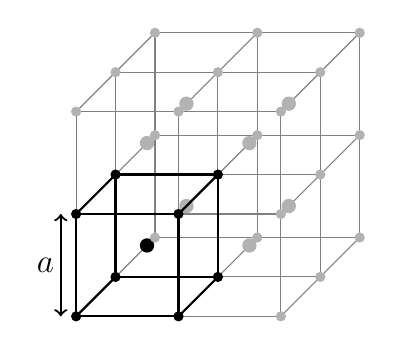
\begin{tikzpicture}[scale=1.3]

                    % 色の設定
                    \definecolor{lightgray}{rgb}{0.7, 0.7, 0.7}
                    \definecolor{gray}{rgb}{0.5, 0.5, 0.5}
                    \draw[red] (0, 0, 0); 
                    % 立方体のエッジ（全体を薄緑色で描画）
                    \foreach \x in {0,...,2}
                        \foreach \y in {0,...,2}{
                            \draw[gray] (\x,\y,0) -- ++(0,0,2);
                            \draw[gray] (0,\x,\y) -- ++(2,0,0);
                            \draw[gray] (\x,0,\y) -- ++(0,2,0);
                        }

                    % 体心の原子 (中央に配置、手前の立方体は黒、それ以外は灰色)
                    \foreach \x in {0.5,1.5}
                        \foreach \y in {0.5,1.5}
                            \foreach \z in {0.5,1.5} {
                                \pgfmathparse{int(\x==0.5 && \y==0.5 && \z==1.5)}
                                \ifnum\pgfmathresult=1
                                    \fill[black, thick] (\x,\y,\z) circle (0.07); % 手前の体心原子は黒
                                \else
                                    \fill[lightgray] (\x,\y,\z) circle (0.07); % その他の体心原子は白っぽい灰色
                                \fi
                            }

                    % 頂点の原子 (手前の立方体は黒、それ以外は白っぽい色)
                    \foreach \x in {0,1,2}
                        \foreach \y in {0,1,2}
                            \foreach \z in {0,1,2} {
                                \pgfmathparse{int(\x<2 && \y<2 && 1<=\z)}
                                \ifnum\pgfmathresult=1
                                    \fill[black, thick] (\x,\y,\z) circle (0.05); % 手前の立方体の頂点は黒
                                \else
                                    \fill[lightgray] (\x,\y,\z) circle (0.05); % その他の頂点は白っぽい灰色
                                \fi
                            }

                    % 手前の立方体のエッジを青色で強調
                    \draw[black, thick] (0,0,2) -- (1,0,2) -- (1,1,2) -- (0,1,2) -- cycle;
                    \draw[black, thick] (0,0,1) -- (0,0,2);
                    \draw[black, thick] (1,0,1) -- (1,0,2);
                    \draw[black, thick] (1,1,1) -- (1,1,2);
                    \draw[black, thick] (0,1,1) -- (0,1,2);
                    \draw[black, thick] (0,0,1) -- (1,0,1) -- (1,1,1) -- (0,1,1) -- cycle;

                    % 垂直方向（高さの辺）
                    \draw[thick, <->] (-0.15, 0, 2) -- (-0.15, 1, 2); 
                    \node at (-0.30, 0.5, 2) {\large $a$};

                \end{tikzpicture}
            \end{center}
        \item[\egg{4}] 下の図のように, ~関数 \( y = ax^2 \) のグラフ上に3点 \( A, B, C \) がある.
        \( A \) と \( C \) の \( y \) 座標は等しい. ~また, ~直線 \( AB \) は四角形 \( AOBC \) の面積を2等分し, ~その式は  
        \(y = -\frac{1}{2}x + 2\)である.
        \(O\)を通り, ~四角形 \( AOBC \)の面積を2等分する直線の式を求めよ.
        \begin{center}
            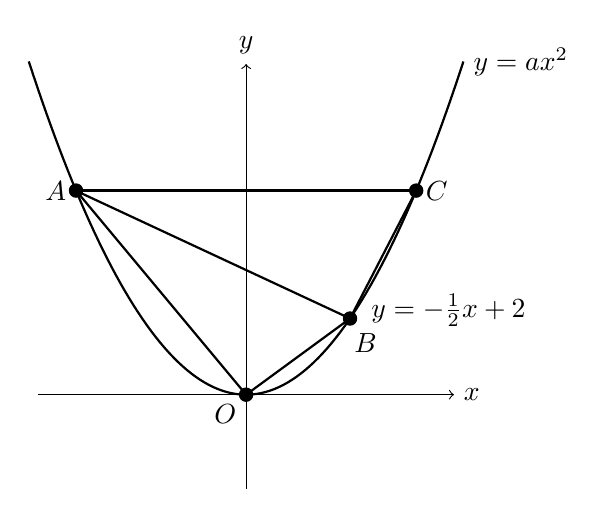
\begin{tikzpicture}[scale=1.2]
                % 座標軸
                \draw[->] (-2.2,0) -- (2.2,0) node[right] {\( x \)};
                \draw[->] (0,-1.0) -- (0,3.5) node[above] {\( y \)};
                
                % 放物線 y = ax^2
                \draw[thick, domain=-2.3:2.3, samples=100] 
                    plot (\x, {2*\x*\x/3}) node[right] {\( y = ax^2 \)};
        
                % 点A, B, C, O
                \filldraw (-1.8,2.16) circle (2pt) node[left] {\( A \)};
                \filldraw (1.8,2.16) circle (2pt) node[right] {\( C \)};
                \filldraw (0,0) circle (2pt) node[below left] {\( O \)};
                \filldraw (1.1, 0.806) circle (2pt) node[below right, xshift=-0.2em, yshift=-0.2em] {\( B \)};
        
                % 直線AC, 
                \draw[thick] (-1.8, 2.16) -- (1.8, 2.16);
                % 直線AO
                \draw[thick, domain=-1.8:0.0]
                    plot (\x, {-1.2*\x});
                % 直線OB
                \draw[thick, domain=0.0:1.1]
                    plot (\x, {0.7327*\x});
                % 直線BC
                \draw[thick, domain=1.1:1.8]
                    plot (\x, {1.934*\x-1.321});
                % 直線AB
                \draw[thick, domain=-1.8:1.1]
                    plot (\x, {-0.466*\x+1.319}) node[right, xshift=0.4em, yshift=0.3em] {\( y = -\frac{1}{2}x+2 \)};
        
            \end{tikzpicture}
        \end{center}
    \end{enumerate}
\end{adjustwidth}
\clearpage

%-------------------------------問2----------------------
\begin{adjustwidth}{1em}{0em} 
    \raggedright
    \noindent\textbf{問\hspace{0.5em}2} \hspace{0.5em}
    次の画像は, ~第2期第四話において登場人物同士がコードネームで呼び合う場面の一部である。
    以下のA \textasciitilde\;Dに示す登場人物の本名に対応するコードネームとして最も適当なものを, ~次の
    \!\egg{1}\textasciitilde\!\egg{9}のうちから一つずつ選べ。
    必要ならば\;\hyperlink{page.13}{「キャラクター一覧」}\;を参考にしてもよい。
    \counterbox[-0.20em]\hspace{4.0em}\raisebox{-1.3px}{〜}\hspace{0.4em}\addtocounter{boxcounter}{2}\counterbox[-0.20em]\hspace{4.0em}\\[1.6em]

    \captionsetup{skip=0pt}
    \begin{figure}[htbp]
        \centering
        \begin{minipage}[C]{0.55\textwidth} % 画像と同じ幅のminipageを作る
            \centering
            \includegraphics[width=\textwidth, trim=0cm 9cm 0cm 9cm, clip]{ansatu_codename2_gray.pdf}
            \captionsetup{labelformat=empty}
            % \caption{\raisebox{5em}{第2期第四話「紡ぐ時間」から引用}}
            \caption{第2期第四話「紡ぐ時間」より}
        \end{minipage}
    \end{figure}
\end{adjustwidth}
\addtocounter{boxcounter}{-4}
\vspace{1.5em}
\newcommand{\ibf}[1]{\textbf{#1}\hspace{0.5em}}
\begin{tabularx}{\textwidth}{l l @{\hspace{7em}} l}  % 3列を均等にする
    \ibf{A} 赤羽業  & \counterbox & \fbox{%
        \newcommand{\iibf}[1]{\!\egg{#1}\!}
        \iibf{1}\iibf{2}\iibf{3}\iibf{4}\iibf{5}\iibf{6}\iibf{7}\iibf{8}\iibf{9}
    }\\[0.5em]
    \ibf{B} 潮田渚  & \counterbox & \fbox{%
        \newcommand{\iibf}[1]{\!\egg{#1}\!}
        \iibf{1}\iibf{2}\iibf{3}\iibf{4}\iibf{5}\iibf{6}\iibf{7}\iibf{8}\iibf{9}
    }\\[0.5em]
    \ibf{C} 寺坂竜馬  & \counterbox & \fbox{%
        \newcommand{\iibf}[1]{\!\egg{#1}\!}
        \iibf{1}\iibf{2}\iibf{3}\iibf{4}\iibf{5}\iibf{6}\iibf{7}\iibf{8}\iibf{9}
    }\\[0.5em]
    \ibf{D} 吉田大成  & \counterbox & \fbox{%
        \newcommand{\iibf}[1]{\!\egg{#1}\!}
        \iibf{1}\iibf{2}\iibf{3}\iibf{4}\iibf{5}\iibf{6}\iibf{7}\iibf{8}\iibf{9}
    }\\[0.5em]
\end{tabularx}
\par
\vspace{3.0em}
\addtocounter{boxcounter}{-4}
\hspace{-2.0em}\counterbox[-0.10em]\hspace{4.0em}\text{〜}\hspace{0.4em}\addtocounter{boxcounter}{2}\counterbox[-0.10em]\hspace{4.0em}
\text{の解答群}
\vspace{0.8em}
\begin{center}
    \hspace{-2.0em}
    \makebox[\textwidth]{
        \newcommand{\iibf}[1]{\!\egg{#1}\!}
        \renewcommand{\arraystretch}{1.5}  % セルの縦方向の余白を増やす
        \begin{tabular}{|c l c l c l|}
            \hline
            \iibf{1} & 野球バカ  & \iibf{2} & 鷹岡もどき & \iibf{3} & コロコロ上がり \\ 
            \iibf{4} & 中二半  & \iibf{5} & すごいサル  & \iibf{6} & 女たらしクソ野郎 \\ 
            \iibf{7} & 性別  & \iibf{8} & ホームベース  & \iibf{9} & 変態終末期 \\
            \hline
        \end{tabular}
    }
\end{center}
\clearpage 
% ---------------------------------------------------------3---------------------------------
\nextmondai
以下のグラフおよび図は, ~あるアニメに関するものである。
これらの内容に基づいて\(X\)に入る最も適当な記号を, ~次の
\!\egg{1}\textasciitilde\!\egg{5}のうちから一つ選べ。
\hspace{0.6em}\counterbox[-0.12em]\hspace{3.8em}\haiten{10}\\[-0.1em]

\begin{center}
    \begin{tikzpicture}[scale=0.9]
        % === データセット定義（\edef の {} を修正）===
        \edef\DataSetA{-0.275349, -0.195284}
        \edef\DataSetB{0.000000, 0.121007, 0.134891, 0.170922, 0.191519, 0.201216, 0.201300, 0.210317, 0.252525, 0.295582, 0.328403, 0.334581, 0.337161, 0.337187, 0.337187, 0.337187, 0.337199, 0.337337, 0.338249, 0.369432, 0.409420, 0.409420, 0.409431, 0.456903, 0.456903, 0.456904, 0.456914, 0.456914, 0.456914, 0.456919, 0.456923, 0.500000, 0.509736, 0.523291, 0.523299, 0.523299, 0.523301, 0.523307, 0.523307, 0.549111, 0.571015, 0.571024, 0.571046, 0.571082, 0.615483, 0.733277, 0.751354}
        \edef\DataSetC{1.053649, 1.055821, 1.064750, 1.064756, 1.081163, 1.097302, 1.123581, 1.129848, 1.129954, 1.130204, 1.130205, 1.130205, 1.130207, 1.130209, 1.130209, 1.130212, 1.130238, 1.130426, 1.130426, 1.130427, 1.143688, 1.382733, 1.467093, 1.703129, 1.818520}
        \edef\DataSetD{2.015105, 2.224529, 2.615074}
        \edef\DataSetE{3.019430, 3.030493, 3.130238, 3.182879, 3.372329, 3.386019, 3.406288, 3.600104, 3.667293}
        \edef\DataSetF{4.034591, 4.389117, 4.456441, 4.456442, 4.493623, 4.493624, 4.530805, 4.530806}
    
        % 軸の描画
        \draw[->] (-1.0, 0) -- (12, 0); % 横軸
        \draw[->] (0, -1.5) -- (0, 6.5);  % 縦軸
    
        \foreach \y in {1.000000,2.000000,3.000000,4.000000} {
            % 目盛り線 (これはそのまま)
            \draw (-0.17, 1.3*\y) -- (0.17, 1.3*\y);
        }
        % 縦軸のメモリとラベル
        \begin{scope}[shift={(0,0)}] % ← ここで左側にずらす
            \foreach \y in {1.000000,2.000000,3.000000,4.000000} {
                % ラベルだけを別のスコープで左へ
                \node[left, transform canvas={xshift=-0.1em}] at (-0.17, 1.3*\y) {\y};
            }
        \end{scope}

        % 縦線（点線）で領域分割
        \draw[dashed] (0.5, -1.5) -- (0.5, 6.5);
        \draw[dashed] (4.6, -1.5) -- (4.6, 6.5);
        \draw[dashed] (8.0, -1.5) -- (8.0, 6.5);
        \draw[dashed] (8.5, -1.5) -- (8.5, 6.5);
        \draw[dashed] (10.1, -1.5) -- (10.1, 6.5);

        \node[draw=none] at (0.25, -1.8) {\large $\Omega$};
        \node[draw=none] at (2.5, -1.8) {\large $\alpha$};
        \node[draw=none] at (6.3, -1.8) {\large $\beta$};
        \node[draw=none] at (8.22, -1.8) {\large $\gamma$};
        \node[draw=none] at (9.35, -1.8) {\large $\delta$};
        \node[draw=none] at (11.1, -1.8) {\large $\epsilon$};

        \draw[semithick, <->] (0.0, -1.2) -- (0.5, -1.2);
        \draw[semithick, <->] (0.5, -1.2) -- (4.6, -1.2);
        \draw[semithick, <->] (4.6, -1.2) -- (8.0, -1.2);
        \draw[semithick, <->] (8.0, -1.2) -- (8.5, -1.2);
        \draw[semithick, <->] (8.5, -1.2) -- (10.1, -1.2); 
        \draw[semithick, <->] (10.1, -1.2) -- (12.0, -1.2); 

        % データセットの要素数をカウント
        % \newcount\DataSize
        % \newcommand{\CountData}[1]{%
        %     \DataSize=0
        %     \foreach \i in {#1} {%
        %         \addtocounter{DataSize}{1}
        %     }%
        % }

        % データセット A (範囲 0.2 ~ 1.8)
        \foreach \i [count=\j from 0] in \DataSetA {
            \pgfmathparse{0.1 + \j * (0.5 - 0.1)/1}
            \let\xA\pgfmathresult
            \pgfmathsetmacro\yA{1.3*\i}
            \filldraw[black] (\xA, \yA) circle (1pt);

            \ifnum\j>0
                \draw[thick, gray] (\prevX, \prevY) -- (\xA, \yA);
            \fi

            \xdef\prevX{\xA}
            \xdef\prevY{\yA}
        }

        % データセット B (範囲 2.2 ~ 3.8)
        \foreach \i [count=\j from 0] in \DataSetB {
            \pgfmathparse{0.5 + \j * (4.6 - 0.5)/(46)}
            \let\xB\pgfmathresult
            \filldraw[black] (\xB, 1.3*\i) circle (1pt);

            \ifnum\j>0
                \draw[thick, gray] (\prevX, \prevY) -- (\xB, 1.3*\i);
            \fi

            \xdef\prevX{\xB}
            \xdef\prevY{1.3*\i}
        }

        % % データセット C (範囲 4.2 ~ 5.8)
        \foreach \i [count=\j from 0] in \DataSetC {
            \pgfmathparse{4.6 + \j * (8.0 - 4.6)/24}
            \let\xC\pgfmathresult
            \filldraw[black] (\xC, 1.3*\i) circle (1pt);

            \ifnum\j>0
                \draw[thick, gray] (\prevX, \prevY) -- (\xC, 1.3*\i);
            \fi

            \xdef\prevX{\xC}
            \xdef\prevY{1.3*\i}
        }

        % データセット D (範囲 6.2 ~ 7.8)
        \foreach \i [count=\j from 0] in \DataSetD {
            \pgfmathparse{8.0 + \j * (8.5 - 8.0)/2}
            \let\xD\pgfmathresult
            \filldraw[black] (\xD, 1.3*\i) circle (1pt);

            \ifnum\j>0
                \draw[thick, gray] (\prevX, \prevY) -- (\xD, 1.3*\i);
            \fi

            \xdef\prevX{\xD}
            \xdef\prevY{1.3*\i}
        }

        % % データセット E (範囲 8.2 ~ 9.8)
        \foreach \i [count=\j from 0] in \DataSetE {
            \pgfmathparse{8.5 + \j * (10.1 - 8.5)/(8)}
            \let\xE\pgfmathresult
            \filldraw[black] (\xE, 1.3*\i) circle (1pt);

            \ifnum\j>0
                \draw[thick, gray] (\prevX, \prevY) -- (\xE, 1.3*\i);
            \fi

            \xdef\prevX{\xE}
            \xdef\prevY{1.3*\i}
        }

        % % データセット F (範囲 10.2 ~ 11.8)
        \foreach \i [count=\j from 0] in \DataSetF {
            \pgfmathparse{10.1 + \j * (11.9 - 10.1)/(7)}
            \let\xF\pgfmathresult
            \filldraw[black] (\xF, 1.3*\i) circle (1pt);

            \ifnum\j>0
                \draw[thick, gray] (\prevX, \prevY) -- (\xF, 1.3*\i);
            \fi

            \xdef\prevX{\xF}
            \xdef\prevY{1.3*\i}
        }
        \node[anchor=south west] at ([shift={(-0.2,0.85)}]current bounding box.north west) {\Large グラフ};
    \end{tikzpicture}
\end{center}
\vspace{0.7em}
\begin{center}
    \begin{tikzpicture}
        % 各期間の枠
        \node[draw, rectangle, minimum width=2.5cm, minimum height=1cm, semithick, align=center] (WW1) at (0,0) {\large 1914\;\textasciitilde\;1918};
        \node[draw, rectangle, minimum width=2.5cm, minimum height=1cm, semithick, align=center] (WW2) at (5.0,0) {\large1939\;\textasciitilde\;1945};
        \node[draw, rectangle, minimum width=2.5cm, minimum height=1cm, semithick] (Modern) at (10,0) {\hspace{-1.2em}\large 2015\;\textasciitilde};
        \node[draw, dashed, rectangle, minimum width=4.6cm, minimum height=2.5cm, anchor=east] (ModernDash) at ($(Modern.east) + (0.5,0)$) {};
        \node[draw=none] at ($(WW2.east) + (1.1,0.4)$) {\Large $X$};
        % \node[draw=none, fill=white] at ($(ModernDash.north) + (0,0)$) {\large $\beta$};
        % 矢印で接続
        \draw[very thick, ->]  
            ($(WW1.east) + (0.1,0) $) -- ($ (WW2.west) - (0.1,0)$);
        \draw[very thick, ->]
            ($(WW2.east) + (0.1, 0)$) -- ($(Modern.west) - (0.1, 0)$);

        \node[anchor=south west] at ([shift={(-1,0.3)}]current bounding box.north west) {\Large 図};
    \end{tikzpicture}
\end{center}
\vspace{2.5em}
\begin{center}
    \makebox[\textwidth][r]{
        \newcommand{\iibf}[1]{\!\egg{#1}\;\:}
        \renewcommand{\arraystretch}{1.5}  % セルの縦方向の余白を増やす
        \begin{tabularx}{\textwidth}{|X X X X X|}
            \hline
            \iibf{1} \large $\Omega$  & \iibf{2} \large $\alpha$  & \iibf{3} \large $\beta$ & \iibf{4} \large $\gamma$ & \iibf{5} \large $\delta$ \\
            \hline
        \end{tabularx}
    }
\end{center}

\clearpage 
% ----------------------------------------------------------4--------------------------------
\nextmondai
集合に関する以下の問いに答えよ。\haiten{16}\\[1.5em]
\noindent\textbf{問\hspace{0.5em}1} \hspace{0.5em} 
以下のベン図が与えられたとき, ~次の要素\:I \textasciitilde ~IIIの分類として最も適当なものを, ~次の
\!\egg{1}\!\textasciitilde\!\egg{8}のうちから１つ選べ。\counterbox[-0.12em]

\begin{center}
    \begin{tikzpicture}
        % 全体集合 U（長方形の左上の辺を削除）
        \draw[thick] (-5.5,4) -- (7,4) -- (7,-4) -- (-7,-4) -- (-7, 4) -- (-6.0, 4);
        % \draw[->] (-6,0) -- (6, 0);
        % \draw[->] (0,-3) -- (0, 4);
        % U のラベルを左上に配置
        \node[draw=none, fill=beige] at (-5.8,4) {\LARGE $U$};
        % 集合 A（円の北西部分を削除）
        \draw[thick] (-0.1,2.3) arc[start angle=140, end angle=480, radius=3.6];
        % A のラベルを削除部分に配置
        \node[draw=none, fill=beige] at (0.35,2.9) {\LARGE $A$};
        % Aでない要素
        \node[draw=none, fill=beige] at (-4.0, 3.0) {\large 土間大平};
        \node[draw=none, fill=beige] at (-4.0, 2.0) {\large エミリア（リゼロ）};
        \node[draw=none, fill=beige] at (-4.0, 1.0) {\large ナツキ・スバル};
        \node[draw=none, fill=beige] at (-4.0, 0.0) {\large 岩谷尚文};
        \node[draw=none, fill=beige] at (-4.0, -1.0) {\large 毛利蘭};
        \node[draw=none, fill=beige] at (-4.0, -2.0) {\large ミカサ・アッカーマン};
        \node[draw=none, fill=beige] at (-3.7, -3.0) {\large リヴァイ・アッカーマン};
        % Aの要素
        \node[draw=none, fill=beige] at (2.4, 2.2) {\large 土間埋};
        \node[draw=none, fill=beige] at (2.4, 1.2) {\large パック（リゼロ）};
        \node[draw=none, fill=beige] at (2.4, 0.2) {\large フィーロ（盾の勇者）};
        \node[draw=none, fill=beige] at (2.4, -0.8) {\large 江戸川コナン};
        \node[draw=none, fill=beige] at (2.5, -1.8) {\large エレン・イェーガー};
    \end{tikzpicture}
\end{center}
\vspace{3em}
% \newcommand{\ibf}[1]{\text{#1}\hspace{0.5em}}
\begin{tabularx}{\textwidth}{X X X}  % 3列を均等にする
    \ibf{I} 綾小路清隆  & \ibf{II} 竈門禰󠄀豆子  & \ibf{III} 御坂美琴 \\[0.8em]
\end{tabularx}
\par
\vspace{1em}

\begin{center}
    \hspace{-2.0em}
    \centering
    \makebox[\textwidth]{
        \newcommand{\iibf}[1]{\!\!\egg{#1}\!}
        \renewcommand{\arraystretch}{1.5}
        \begin{tabularx}{0.71\textwidth}{|c|c|c|c|c|c|c|c|c|}
            \hline
            &\iibf{1}&\iibf{2}&\iibf{3}&\iibf{4}&\iibf{5}&\iibf{6}&\iibf{7}&\iibf{8}\\ 
            \hline
            \;\ibf{I}\!& \large \(A\) & \large \(A\) & \large \(A\) & \large \(A\) 
            & \large \(\widebar{A}\) & \large \(\widebar{A}\) & \large \(\widebar{A}\) & \large \(\widebar{A}\)\\
            \hline
            \;\ibf{II}\!& \large \(A\) & \large \(A\) & \large \(\widebar{A}\) & \large \(\widebar{A}\)
            & \large \(A\) & \large \(A\) & \large \(\widebar{A}\) & \large \(\widebar{A}\)\\
            \hline
            \;\ibf{III}\!& \large \(A\) & \large \(\widebar{A}\) & \large \(A\) & \large \(\widebar{A}\) 
            & \large \(A\) & \large \(\widebar{A}\) & \large \(A\) & \large \(\widebar{A}\)\\
            \hline
        \end{tabularx}
    }
\end{center}
\clearpage
%--------問2------------
\noindent\textbf{問\hspace{0.5em}2} \hspace{0.5em} 
以下のベン図が与えられたとき, ~次の要素\:I \textasciitilde ~IIIの分類として最も適当なものを
\!\egg{1}\textasciitilde\!\egg{4}のうちから１つずつ選べ。\\
\counterbox[-0.20em]\hspace{4.0em}\text{〜}\hspace{0.4em}\addtocounter{boxcounter}{1}\counterbox[-0.20em]\hspace{4.0em}
\vspace*{2em}
\begin{center}
    \begin{tikzpicture}[scale=0.92]
        % 全体集合 U（長方形の左上の辺を削除）
        \draw[thick] (-6.0,5) -- (6,5) -- (6,-5) -- (-8,-5) -- (-8, 5) -- (-6.5, 5);
        % \draw[->] (-6,0) -- (6, 0);
        % \draw[->] (0,-3) -- (0, 4);
        % U のラベルを左上に配置
        \node[draw=none, fill=beige] at (-6.3,5) {\LARGE $U$};
        % 集合 A（円の北西部分を削除）
        \draw[thick] (-6.4,2.3) arc[start angle=140, end angle=480, radius=4.1];
        \draw[thick] (3.4,3.2) arc[start angle=60, end angle=400, radius=4.1];
        % A のラベルを削除部分に配置
        \node[draw=none, fill=beige] at (-5.9,3.0) {\LARGE $A$};
        \node[draw=none, fill=beige] at (4.1,2.9) {\LARGE $B$};
        % Aの要素
        \node[draw=none, fill=beige] at (-4.7, 2.0) {\large アーニャ};
        \node[draw=none, fill=beige] at (-4.7, 1.0) {\large 後藤ひとり};
        \node[draw=none, fill=beige] at (-4.7, 0.0) {\large 藤原千花};
        \node[draw=none, fill=beige] at (-4.7, -1.0) {\large 鹿目まどか};
        \node[draw=none, fill=beige] at (-4.7, -2.0) {\large 芳岡ユイ};
        \node[draw=none] at (-4.05, -3.0) {\large ラム（リゼロ）};
        % Bの要素
        \node[draw=none, fill=beige] at (2.4, 1.8) {\large 坂上智代};
        \node[draw=none, fill=beige] at (2.4, 0.8) {\large 川嶋亜美};
        \node[draw=none, fill=beige] at (2.8, -0.2) {\large 小林カンナ};
        \node[draw=none, fill=beige] at (2.75, -1.2) {\large 暁美ほむら};
        \node[draw=none, fill=beige] at (2.4, -2.2) {\large 蛇喰夢子};
        % AとBの要素
        \node[draw=none, fill=none] at (-1.0, 1.0) {\large 中野一花};
        \node[draw=none] at (-1.1, -0.45) {\large 各務原};
        \node[draw=none] at (-1.1, -1.0) {\large なでしこ};
    \end{tikzpicture}
\end{center}
\vspace{1em}
\addtocounter{boxcounter}{-3}
\begin{tabularx}{\textwidth}{c l l @{\hspace{8em}} l}  % 3列を均等にする
    \ibf{I} &椎名真昼  & \counterbox & \fbox{%
        \newcommand{\iibf}[1]{\!\egg{#1}\!}
        \iibf{1}\iibf{2}\iibf{3}\iibf{4}
    }\\[0.75em]
    \ibf{II} &西森柚咲  & \counterbox & \fbox{%
        \newcommand{\iibf}[1]{\!\egg{#1}\!}
        \iibf{1}\iibf{2}\iibf{3}\iibf{4}
    }\\[0.75em]
    \ibf{III} &楪いのり  & \counterbox & \fbox{%
        \newcommand{\iibf}[1]{\!\egg{#1}\!}
        \iibf{1}\iibf{2}\iibf{3}\iibf{4}
    }\\[0.75em]
\end{tabularx}
\par
\vspace{1.5em}
\addtocounter{boxcounter}{-3}
\counterbox[-0.10em]\hspace{4.0em}\text{〜}\hspace{0.4em}\addtocounter{boxcounter}{1}\counterbox[-0.10em]\hspace{4.0em}
\text{の解答群（同じものを繰り返し選んでもよい。）}
\vspace{0.8em}

\begin{center}
    \hspace{-1.0em}
    \makebox[\textwidth]{
        \newcommand{\iibf}[1]{\!\egg{#1}\;\:}
        \renewcommand{\arraystretch}{1.5}  % セルの縦方向の余白を増やす
        \newcommand{\caap}{\,\scalebox{1.3}{$\cap$}\,}
        \begin{tabularx}{\textwidth}{|X X X X|}
            \hline
            \iibf{1} \(A \caap B\)  & \iibf{2} \(\widebar{A} \caap B\) &
            \iibf{3} \(A \caap \widebar{B}\) & \iibf{4} \(\widebar{A} \caap \widebar{B}\)\\ 
            \hline
        \end{tabularx}
    }
\end{center}

\clearpage 
% -----------------------------------------------------------5-------------------------------
\nextmondai
以下の問1\:\textasciitilde\:問3の下線部の漢字に相当する読みとして最も適当なものを,~ 
次の\!\egg{1}\textasciitilde\!\egg{3}のうちから一つずつ選べ。\haiten{10}\\[0.2em]
\begin{adjustwidth}{1em}{0em} 
    \renewcommand{\ULdepth}{5.0pt} 
    \renewcommand{\ULthickness}{1.5pt} 
    \newcommand{\iibf}[1]{\!\egg{#1}\!}
    \definecolor{tmp_col}{RGB}{252, 252, 252}
    \raggedright
    \noindent\textbf{問\hspace{0.5em}1} \hspace{0.5em} \counterbox \\ [1.0em]
    \begin{adjustbox}{minipage=\linewidth} % 横幅調整
        \begin{tcolorbox}[colframe=black, colback=tmp_col, boxrule=0.7pt, arc=0mm]
            {\small 『水素爆弾』の直撃に\textemdash\textemdash すなわち。~太陽コロナをも上回る熱波、50メガトンの衝撃波、
            気体蒸発による酸欠と超滅圧、そして残留する毒物にさえ堪えた\textemdash\textemdash 序列第六位\uline{天翼種}。}
        \end{tcolorbox}
    \end{adjustbox}
    \\
    \vspace{1.3em}
    \begin{tabularx}{\textwidth}{X X X}  % 3列を均等にする
        \iibf{1} イマニティ  & \iibf{2} ファンタズマ  & \iibf{3} フリユーゲル
    \end{tabularx}
    \\
    \vspace{1.5em}
    \noindent\textbf{問\hspace{0.5em}2} \hspace{0.5em} \counterbox\\ [1.0em]
    \begin{adjustbox}{minipage=\linewidth} % 横幅調整
        \begin{tcolorbox}[colframe=black, colback=tmp_col, boxrule=0.7pt, arc=0mm]
            {\small《告。暴食之王による対消滅を進言します。諦めないで下さい 》\;
            幾つもの対抗手段の中、もっとも成功率が高いものを俺に提示してくれる。
            \uline{智慧之王}\:の声に従い暴食之王を起動。}
        \end{tcolorbox}
    \end{adjustbox}
    \\
    \vspace{1.3em}
    \begin{tabularx}{\textwidth}{X X X}  % 3列を均等にする
        \iibf{1} ガブリエル  & \iibf{2} メタトロン  & \iibf{3} ラファエル
    \end{tabularx}
    \\
    \vspace{1.5em}
    \noindent\textbf{問\hspace{0.5em}3} \hspace{0.5em} \counterbox\\ [1.0em]
    \begin{adjustbox}{minipage=\linewidth} % 横幅調整
        \begin{tcolorbox}[colframe=black, colback=tmp_col, boxrule=0.7pt, arc=0mm]
            {\small \uline{超能力者}\:用の付帯施設は、彼女の在籍している常盤台中学の敷地に
            奇麗にまとめられているとは限らない。
            中には学校の敷地から離れた『飛び地』に出向かなければならない事もある。
            }
        \end{tcolorbox}
    \end{adjustbox}
    \\
    \vspace{1.3em}
    \begin{tabularx}{\textwidth}{X X X}  % 3列を均等にする
        \iibf{1} レベル1 & \iibf{2} レベル5  & \iibf{3} レベル6
    \end{tabularx}
\end{adjustwidth}

\clearpage 
% ------------------------------------------------------------6------------------------------
\nextmondai
画像I\;\textasciitilde\;VIについて, ~関係式\:
\(
\textbf{「}\text{\:I} < \text{II} = \text{III} < \text{IV} < \text{V} \ll \text{VI\:}\textbf{」}
\)\:
が成り立っているとき, \;\counterbox[-0.12em]\hspace{4.0em}\text{・}\hspace{0.4em}\counterbox[-0.12em]\hspace{4.0em}\text{に当てはまる記号}\\[0.2em]
として最も適当なものを, ~次の\!\egg{1}\textasciitilde\!\egg{3}のうちから一つずつ選べ。\haiten{10}\\
\addtocounter{boxcounter}{-2}

\begin{tabularx}{\textwidth}{@{\hspace{6em}} l @{\hspace{3em}} l}  % 3列を均等にする
    A\;\,\counterbox[-0.12em]\hspace{4.0em}\text{B} & \raisebox{-0.2em}{\fbox{%
        \newcommand{\iibf}[1]{\!\egg{#1}\!}
        \iibf{1}\iibf{2}\iibf{3}
    }}\\[0.75em]
    C\;\,\counterbox[-0.12em]\hspace{4.0em}\text{D} & \raisebox{-0.2em}{\fbox{%
        \newcommand{\iibf}[1]{\!\egg{#1}\!}
        \iibf{1}\iibf{2}\iibf{3}
    }}\\[0.75em]
\end{tabularx}

% \begin{multicols}{2}
%     \renewcommand{\labelenumi}{}
%     \begin{enumerate}
%         \item A\;\,\counterbox[-0.12em]\hspace{4.0em}\text{B}
%         \item C\;\,\counterbox[-0.12em]\hspace{4.0em}\text{D}
%     \end{enumerate}
% \end{multicols}
\begin{figure}[htbp]
    \captionsetup[subfigure]{labelformat=empty} 
    \begin{adjustbox}{scale=0.43, center}
        \subfloat[]{
            \begin{tikzpicture}
                \node[anchor=north west] (img) at (0,0) {\includegraphics[scale=0.28]{akusera.png}};
                \node[anchor=north west, xshift=-2pt, yshift=10pt] at (img.north west) {\huge\textbf{I}};
            \end{tikzpicture}
        }
        \hspace*{1em}
        \subfloat[]{
            \begin{tikzpicture}
                \node[anchor=north west] (img) at (0,0) {\includegraphics[scale=0.3]{yotuba3.png}};
                \node[anchor=north west, xshift=-2pt, yshift=10pt] at (img.north west) {\huge\textbf{II}};
            \end{tikzpicture}
        }
        \hspace*{1em}
        \subfloat[]{
            \begin{tikzpicture}
                \node[anchor=north west] (img) at (0,0) {\includegraphics[scale=0.19]{sinomiya.png}};
                \node[anchor=north west, xshift=-2pt, yshift=10pt] at (img.north west) {\huge\textbf{III}};
            \end{tikzpicture}
        }
        \hspace*{1em}
        \subfloat[]{
            \begin{tikzpicture}
                \node[anchor=north west] (img) at (0,0) {\includegraphics[scale=0.21]{nanakusa.png}};
                \node[anchor=north west, xshift=-2pt, yshift=10pt] at (img.north west) {\huge\textbf{IV}};
            \end{tikzpicture}
        }
        \hspace*{1em}
        \subfloat[]{
            \begin{tikzpicture}
                \node[anchor=north west] (img) at (0,0) {\includegraphics[scale=0.21]{yanami.png}};
                \node[anchor=north west, xshift=-2pt, yshift=10pt] at (img.north west) {\huge\textbf{V}};
            \end{tikzpicture}
        }
        \hspace*{1em}
        \subfloat[]{
            \begin{tikzpicture}
                \node[anchor=north west] (img) at (0,0) {\includegraphics[scale=0.35]{titanda.png}};
                \node[anchor=north west, xshift=-2pt, yshift=10pt] at (img.north west) {\huge\textbf{VI}};
            \end{tikzpicture}
        }
    \end{adjustbox}
\end{figure}
\vspace{-2.5em}
\begin{figure}[htbp]
    \captionsetup[subfigure]{labelformat=empty} 
    \begin{adjustbox}{scale=0.43, center}
        \subfloat[]{
            \begin{tikzpicture}
                \node[anchor=north west] (img) at (0,0) {\includegraphics[scale=0.26]{gozyou2.png}};
                \node[anchor=north west, xshift=-2pt, yshift=10pt] at (img.north west) {\huge\textbf{A}};
            \end{tikzpicture}
        }
        \hspace{1.5em}
        \subfloat[]{
            \begin{tikzpicture}
                \node[anchor=north west] (img) at (0,0) {\includegraphics[scale=0.20]{igarashi.png}};
                \node[anchor=north west, xshift=-2pt, yshift=10pt] at (img.north west) {\huge\textbf{B}};
            \end{tikzpicture}
        }
        \hspace{1.5em}
        \subfloat[]{
            \begin{tikzpicture}
                \node[anchor=north west] (img) at (0,0) {\includegraphics[scale=0.27]{issiki3.png}};
                \node[anchor=north west, xshift=-2pt, yshift=10pt] at (img.north west) {\huge\textbf{C}};
            \end{tikzpicture}
        }
        \hspace{1.5em}
        \subfloat[]{
            \begin{tikzpicture}
                \node[anchor=north west] (img) at (0,0) {\includegraphics[scale=0.18]{itinose.png}};
                \node[anchor=north west, xshift=-2pt, yshift=10pt] at (img.north west) {\huge\textbf{D}};
            \end{tikzpicture}
        }
    \end{adjustbox}
\end{figure}

\vspace{0.8em}
\addtocounter{boxcounter}{-2}
\counterbox[-0.10em]\hspace{4.0em}\text{・}\hspace{0.4em}\counterbox[-0.10em]\hspace{4.0em}
\vspace{0.5em}
\text{の解答群（同じものを繰り返し選んでもよい。）}
\begin{center}
    \hspace{-2.0em}
    \makebox[\textwidth]{
        \newcommand{\iibf}[1]{\!\egg{#1}\;\:}
        \renewcommand{\arraystretch}{1.5}  % セルの縦方向の余白を増やす
        \begin{tabularx}{0.95\textwidth}{|X X X|}
            \hline
            \iibf{1} \textbf{<}  & \iibf{2} \textbf{=} & \iibf{3} \textbf{>} \\ 
            \hline
        \end{tabularx}
    }
\end{center}
\clearpage 
% -------------------------------------------------------------7-----------------------------
\nextmondai 
以下の文章は, ~あるアニメに関する口コミである。
この内容に該当するアニメとして最も適当なものを, ~次の
\!\egg{1}\textasciitilde\!\egg{4}のうちから一つ選べ。
\counterbox[-0.1em] \hspace{3.5em} \haiten{10}
\vspace*{-1.3em}
\begin{center}
    \begin{tikzpicture} [scale=0.93]
        % コメント 1
        % \renewcommand{\baselinestretch}{0.7}
        \node[draw=black, thick, rectangle, minimum width=10cm, minimum height=3.0cm, inner xsep=10pt, inner ysep=-2pt, text width=13cm, align=left, anchor=north west] (c1) at (0,0) {
            \vspace{3.3em}
            \begin{spacing}{0.95}
                \fontsize{11pt}{14pt}\selectfont
                他の制作会社だったらこんなに面白くなっていなかったのではないでしょうか。
                長ゼリフや長く続く会話劇を飽きることなく魅せるのが本当に上手いと感じます。
                あと、かなり珍しいと思いますがOPはその回で主役となるキャラに合わせて別々のものが作られています。
            \end{spacing}
        };
         % アイコンの黒枠（枠の左上に配置）
        \draw[thick, black] ($(c1.north west) + (0.9,-0.8)$) circle (0.56cm);
         % アイコンを円形にクリッピングして配置
        \begin{scope}
            \clip ($(c1.north west) + (0.9,-0.8)$) circle (0.55cm);
            \node at ($(c1.north west) + (0.9,-0.8)$) {\includegraphics[width=1.3cm]{unknown-icon.png}};
        \end{scope}

        \begin{scope}
            % アイコンの右の位置 (適宜 x方向にずらす)
            \clip ($(c1.north west) + (1.0, -1.1)$) rectangle 
            ($(c1.north west) + (5.1, 0.8) $);
            \node at ($(c1.north west) + (3.0,-0.8)$) {\includegraphics[width=2.7cm]{five-stars.png}};
        \end{scope}

        % コメント 2
        \node[draw=black, thick, rectangle, minimum width=10cm, minimum height=3.0cm, inner xsep=10pt, inner ysep=-2pt, text width=13cm, align=left, anchor=north west] (c1) at (0,-4.2) {
            \vspace{3.3em}
            \begin{spacing}{0.95}
                \fontsize{11pt}{14pt}\selectfont
                妖怪のような幽霊のような存在に苦しめられる少女達を、特異な存在の少年が解決し助けるという話で、
                学園ハーレム恋愛アニメという印象はあまりなかったかな。
                まるでアートのような建造物や街並み。活字や実写を織り交ぜた描写。深みのある長台詞の会話劇。とてもアニメとは思えない作品です。
            \end{spacing}
        };
        \draw[thick, black] ($(c1.north west) + (0.9,-0.8)$) circle (0.56cm);
        \begin{scope}
            \clip ($(c1.north west) + (0.9,-0.8)$) circle (0.55cm);
            \node at ($(c1.north west) + (0.9,-0.8)$) {\includegraphics[width=1.3cm]{unknown-icon.png}};
        \end{scope}
        \begin{scope}
            \clip ($(c1.north west) + (1.0, -1.1)$) rectangle ($(c1.north west) + (5.1, 0.8) $);
            \node at ($(c1.north west) + (3.0,-0.8)$) {\includegraphics[width=2.7cm]{five-stars.png}};
        \end{scope}
        
        % コメント 3
        \node[draw=black, thick, rectangle, minimum width=10cm, minimum height=3.0cm, inner xsep=10pt, inner ysep=-2pt, text width=13cm, align=left, anchor=north west] (c2) at (0,-8.9) {
            \vspace{3.3em}
            \begin{spacing}{0.95}
                \fontsize{11pt}{14pt}\selectfont
                バラバラになってしまいそうだが、独特な作画による世界観が全てを纏めてしまう。
                字幕を出したと思ったら、読む時間を与えず消してしまうなんて、ありえない演出。
                だが、本筋じゃないエピソードですら、変な緊張感をもって画面に見入ってしまう。
            \end{spacing}
        };
        \draw[thick, black] ($(c2.north west) + (0.9,-0.8)$) circle (0.56cm);
        \begin{scope}
            \clip ($(c2.north west) + (0.9,-0.8)$) circle (0.55cm);
            \node at ($(c2.north west) + (0.9,-0.8)$) {\includegraphics[width=1.3cm]{unknown-icon.png}};
        \end{scope}
        \begin{scope}
            \clip ($(c2.north west) + (1.0, -1.1)$) rectangle ($(c2.north west) + (5.1, 0.8) $);
            \node at ($(c2.north west) + (3.0,-0.8)$) {\includegraphics[width=2.7cm]{three-stars.png}};
        \end{scope}
        
        % コメント 4
        \node[draw=black, thick, rectangle, minimum width=10cm, minimum height=3.0cm, inner xsep=10pt, inner ysep=-2pt, text width=13cm, align=left, anchor=north west] (c3) at (0,-13.1) {
            \vspace{3.3em}
            \begin{spacing}{0.95}
                \fontsize{11pt}{14pt}\selectfont
                一話の階段上るシーンからなぜか拒否反応がでました。
                不思議過ぎてついていけない。最初の説明が足りなさすぎ。
                こういう主人公がやたら語って話進めていくようなアニメは自分の好みではない。
            \end{spacing}
        };
        \draw[thick, black] ($(c3.north west) + (0.9,-0.8)$) circle (0.56cm);
        \begin{scope}
            \clip ($(c3.north west) + (0.9,-0.8)$) circle (0.55cm);
            \node at ($(c3.north west) + (0.9,-0.8)$) {\includegraphics[width=1.3cm]{unknown-icon.png}};
        \end{scope}
        \begin{scope}
            \clip ($(c3.north west) + (1.0, -1.1)$) rectangle ($(c3.north west) + (5.1, 0.8) $);
            \node at ($(c3.north west) + (3.0,-0.8)$) {\includegraphics[width=2.7cm]{one-stars.png}};
        \end{scope}
    \end{tikzpicture}
\end{center}
\vspace*{-1em}
\begin{center}
    \hspace*{1.5em}
    \makebox[\textwidth][r]{
        \newcommand{\iibf}[1]{\!\egg{#1}\!}
        \renewcommand{\arraystretch}{1.5} 
         % セルの縦方向の余白を増やす
        \begin{tabularx}{1.05\textwidth}{| X X X l|}
            \hline
            \iibf{1} 化物語 & \iibf{2} 虚構推理 &
            \iibf{3} 呪術廻戦 & \iibf{4} モブサイコ100 \\
            \hline
        \end{tabularx}
    }
\end{center}

\clearpage 
% ----------------------------------------------------------8--------------------------------
\nextmondai
以下の英文は, ~英語版Wikipediaにも掲載されているアニメに関する単語の説明である。~
問1, ~問2, ~問3の説明が意味する単語を, ~
次の\!\egg{1}\textasciitilde\!\egg{4}のうちから一つずつ選べ。\haiten{12} \\[0.1em]
\begin{adjustwidth}{1em}{0em} 
    \raggedright
    \newcommand{\iibf}[1]{\!\egg{#1}\!}
    \noindent\textbf{問\hspace{0.5em}1} \hspace{0.5em} \counterbox \\ [1.0em]
    \begin{adjustbox}{minipage=\linewidth} % 横幅調整
        \begin{tcolorbox}[colframe=black, colback=beige, boxrule=0.7pt, arc=0mm]
            {\spaceskip=0.4em A genre of science or fantasy fiction featuring a protagonist who is transported to or reincarnated in a different,
            strange, or unfamiliar world. Also: an anime, manga, video game, etc., in this genre. Frequently as a modifier.}
        \end{tcolorbox}
    \end{adjustbox}
    \\
    \vspace{1.1em}
    \hspace*{-0.7em}
    \begin{tabularx}{1.06\textwidth}{X X l l}  % 3列を均等にする
        \iibf{1} historical &\hspace*{0.45em} \iibf{2} isekai & \iibf{3} post-apocalyptic  & \iibf{4} supernatural\\
    \end{tabularx}
    \\
    \vspace{3.8em}
    \noindent\textbf{問\hspace{0.5em}2} \hspace{0.5em} \counterbox \\ [1.0em]
    \begin{adjustbox}{minipage=\linewidth} % 横幅調整
        \begin{tcolorbox}[colframe=black, colback=beige, boxrule=0.7pt, arc=0mm]
            {\spaceskip=0.4em A genre in Japanese anime and manga focuses on romantic or deeply emotional relationships
            between female characters. The term used for this genre originates from the Japanese word for a type of flower, symbolizing purity and femininity.
            Stories in this category can range from close friendships with subtle romantic implications to explicitly developed love narratives.}
        \end{tcolorbox}
    \end{adjustbox}
    \\
    \vspace{1.1em}
    \begin{tabularx}{\textwidth}{X X X X}  % 3列を均等にする
        \iibf{1} catgirl & \iibf{2} romcom & \iibf{3} shojo & \iibf{4}yuri \\
    \end{tabularx}
    \\
    \vspace{5.8em}
    \noindent\textbf{問\hspace{0.5em}3} \hspace{0.5em} \counterbox \\ [1.0em]
    \begin{adjustbox}{minipage=\linewidth} % 横幅調整
        \begin{tcolorbox}[colframe=black, colback=beige, boxrule=0.7pt, arc=0mm]
            {\spaceskip=0.4em A type of self-published work, often in manga or novel format, created by independent artists or groups. 
            These works can be original stories or unofficial adaptations of existing characters and settings. 
            They are typically sold at specialized conventions or online platforms. 
            Unlike mainstream publications, these works are usually produced in small print runs and offer greater creative freedom to their creators.}
        \end{tcolorbox}
    \end{adjustbox}
    \\
    \vspace{1.1em}
    \begin{tabularx}{\textwidth}{X X X X}  % 3列を均等にする
        \iibf{1} comiket & \iibf{2} doujinshi  & \iibf{3} lightnovel & \iibf{4} manga\\
    \end{tabularx}
    \\
\end{adjustwidth} 
\clearpage 
% ----------------------------------------------------------9--------------------------------
\nextmondai
以下は~「ノーゲーム・ノーライフ」に登場するあるゲームが行われている場面を描いたものである。
\quad\counterbox[-0.10em]\hspace{4.0em}に当てはまる単語として最も適当なものを, ~
次の\!\egg{1}\textasciitilde\!\egg{4}のうちから一つ選べ。\haiten{10}\\[1.5em]

\addtocounter{boxcounter}{-1}
\begingroup
\spaceskip=0.5em
\fontsize{12pt}{14pt}\selectfont
Sora and dreadless\textsuperscript{*1} Siro overwhelmed driven native executing gods 
since enemies \;\counterbox[-0.12em]\hspace{4.0em} feeblish\textsuperscript{*2} humanity\\
\endgroup
\\
\vspace{1em}
*1 \; dreadless \quad\textemdash\textemdash\textemdash\textemdash\textemdash\textemdash\;\, 恐れを知らない\\[-1.0em]
\hspace{0.2em}*2 \; feeblish \quad\textemdash\textemdash\textemdash\textemdash\textemdash\textemdash\;\, 弱々しい\\
\vspace{3em}

\newcommand{\iibf}[1]{\!\egg{#1}\!}
\begin{tabularx}{\textwidth}{X X X l}  % 3列を均等にする
    \iibf{1}\;despise & \iibf{2}\;overcome  & \hspace*{0.5em}\iibf{3}\;scoff & \iibf{4}\; underestimate
\end{tabularx}



\clearpage
% -------------------------------------------------------------参考-----------------------------
\hspace*{-1.5em}
\textsf{\textbf{\LARGE キャラクター\:一覧}}
\hspace{4em} % 余白を作って
\hyperlink{page.4}{\textcolor{blue}{問題へ戻る}}
\par
\vspace{5em}
\begin{tikzpicture}[remember picture, overlay]
    \node at ([yshift=-10mm]current page.center) {\includegraphics[width=\paperwidth, height=\paperheight, keepaspectratio]{ansatu_itiran.png}};
\end{tikzpicture}

\end{document}
